%!TEX root = ../Master.tex
\section{PID Control} % (fold)
\label{sec:pid_control}

When the robot has to follow a path errors might occur. To remove this error a Proportional Integral Derivative Controller can be used. As illustrated in \autoref{fig:PIDcontroller} the controller consists of three different parts which handle the error in three different ways. In order to explain the PID controller an example is examined. \\

\begin{figure}[h]
\centering
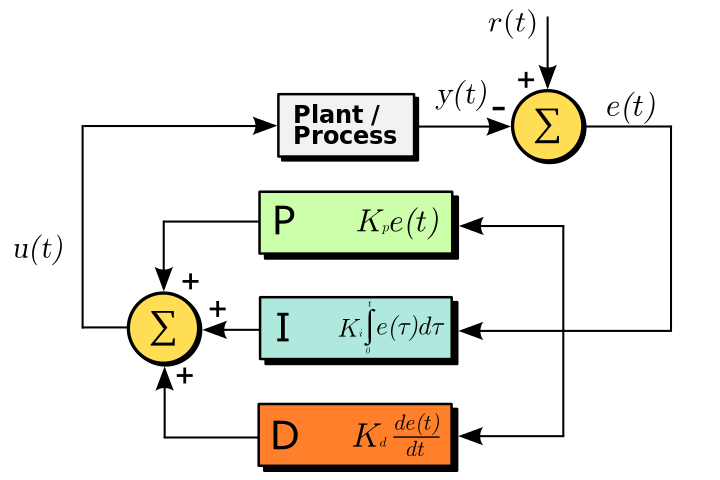
\includegraphics[scale=0.35]{images/PIDController}
\caption{PID controller}
\label{fig:PIDcontroller}
\end{figure}

Imagine a self-driving car trying to follow a path. The car follows the path with an error as illustrated in \autoref{fig:PIDexample}. It is desirable to get the car to follow the path without an error. In order to make that happen the PID controller is used.

\begin{figure}[h]
\centering
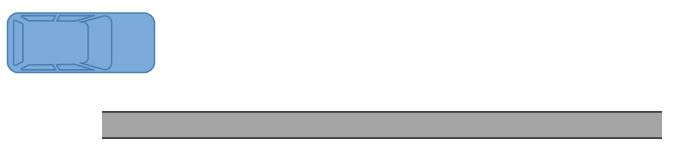
\includegraphics[scale=0.7]{images/PIDexample}
\caption{Self-driving car example}
\label{fig:PIDexample}
\end{figure}

\subsection{Proportional Control} % (fold)
\label{sub:proportional_control}

The proportional part of the PID controller handles the error by using a gain $K_p$ which is proportional with the error. The formula of the output of the proportional controller is shown in \autoref{eq:proportional_controller}.

\begin{equation}
\label{eq:proportional_controller}
u(t)=K_p e(t)
\end{equation}

The proportional controller will try to reduce or eliminate the error. The value of the gain has to be chosen. If the gain is very low the proportional controller reduces the error very slowly. If the gain is very high it might result in a large overshoot or even overdrive which could lead to the car getting out of control. \\

In the example the car should drive along the x-axis with the value of y being equal to 0. Unfortunately the car is driving along the x-axis with the value of y being equal to 1 which means an error of 1. This is illustrated in \autoref{fig:P_controller_example} where all three examples of cars starts in $y=1$ and then tries to correct the error by turning towards $y=0$. \\

\begin{figure}[H]
\centering
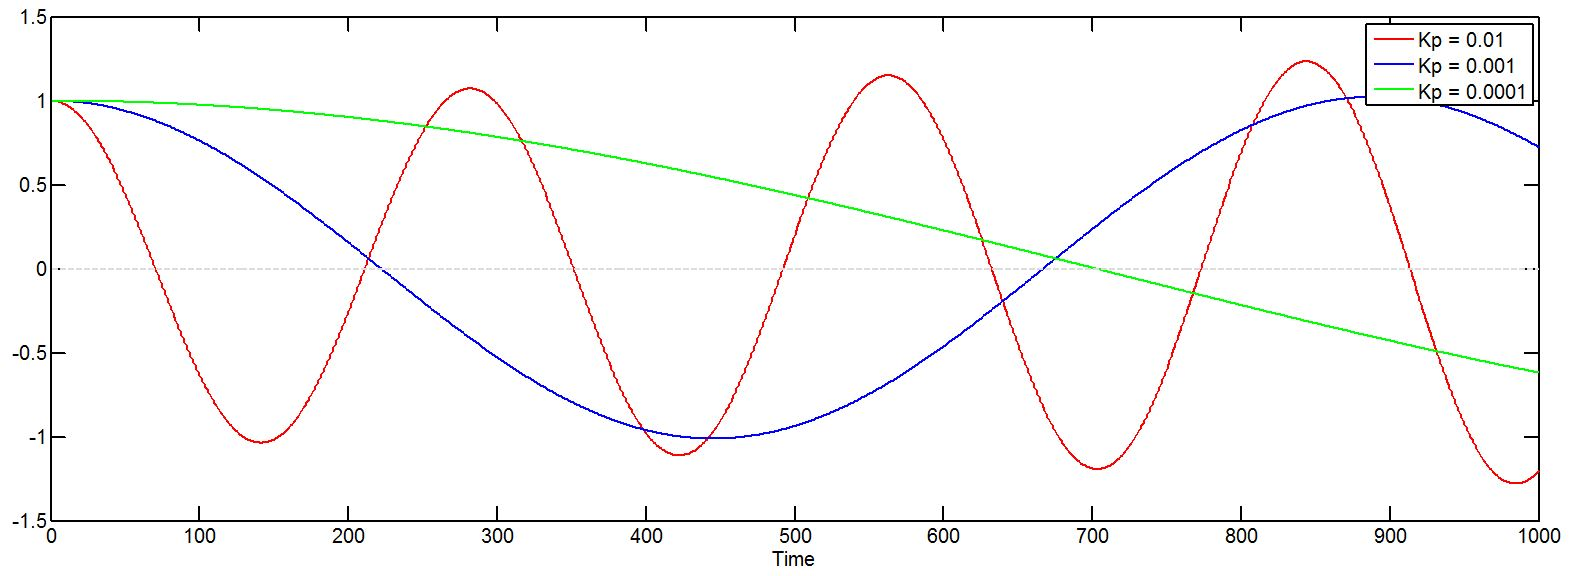
\includegraphics[scale=0.35]{images/Pcontroller.jpg}
\caption{Example of proportional controller}
\label{fig:P_controller_example}
\end{figure}

The highest value of $K_p$ results in the car getting out of control as explained before the illustration. The smallest value results in a very slowly reducing of the error. All $K_p$ values results in overshooting and none of them eliminates the error. \\

% subsection proportional_control (end)

\subsection{Proportional Derivative Control} % (fold)
\label{sub:proportional_derivative_control}

The derivative part of the PID controller handles the error by using a gain $K_d$ which is multiplied by the derivative of the error. This means that it is taking the slope of the error into account. The formula of the output of the derivative controller is shown in \autoref{eq:derivative_controller}.

\begin{equation}
\label{eq:derivative_controller}
u(t)=K_d \frac{de(t)}{dt}
\end{equation}

The derivative controller will try to reduce the overshoot which is caused by the proportional controller. The value of the gain has to be chosen. If the value is very low the derivative controller will not be able to reduce the overshoot. If the value is very high the derivative controller might increase the time it takes for the error to be reduced.\\

In the car example the derivative controller and the proportional controller is combined. The derivative controller reduces or eliminates the overshoot from the proportional controller. The derivative controller also decreases the settling time of the car. This is illustrated in \autoref{fig:PD_controller_example}. \\

\begin{figure}[H]
\centering
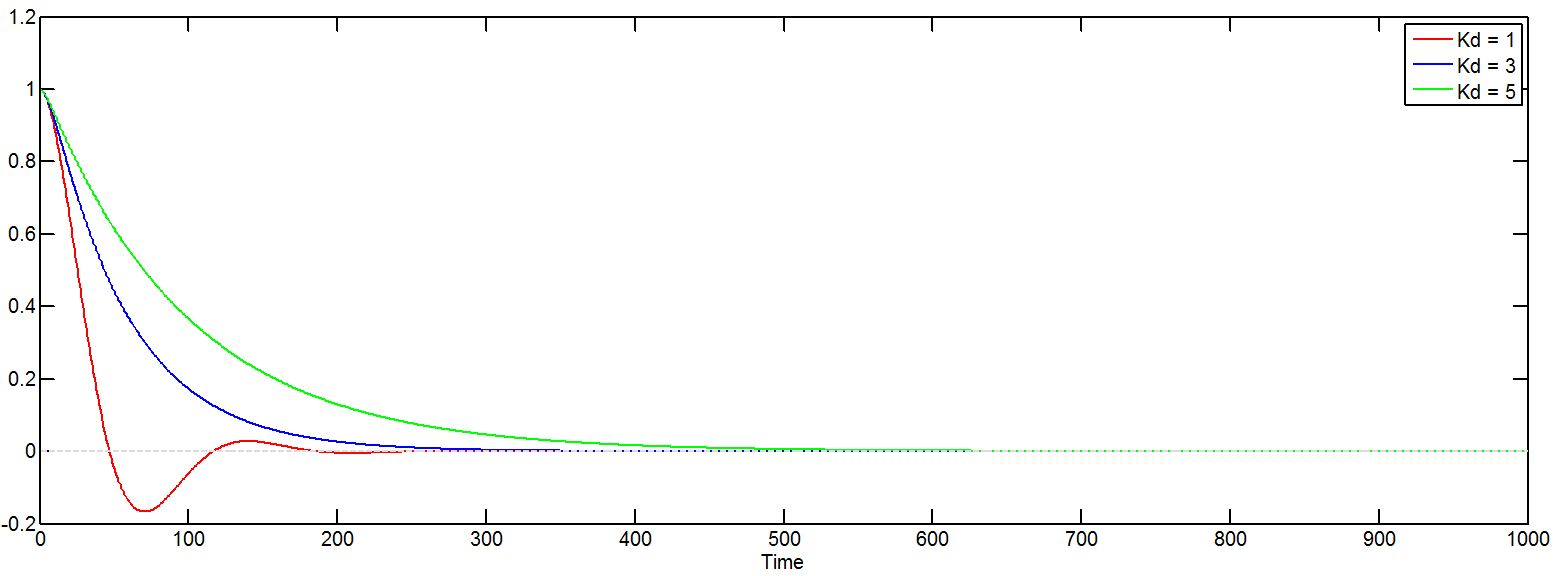
\includegraphics[scale=0.35]{images/PDcontroller.jpg}
\caption{Example of proportional derivative controller}
\label{fig:PD_controller_example}
\end{figure}

The highest value of $K_d$ results in a very slow reduction of the error while the smallest value results in the controller not being able to eliminate the overshoot.

% subsection derivative_control (end)

\subsection{Proportional Integral Derivative Control} % (fold)
\label{sub:integral_control}

The integral part of the controller handles the error by using a gain $K_i$ which is multiplied by the integral of the error. This means that it takes the sum of all errors into account. The formula of the output of the integral controller is shown in \autoref{eq:integral_controller}.

\begin{equation}
\label{eq:integral_controller}
u(t)= K_i \int e(\tau)d\tau
\end{equation}

The integral controller will eliminate a possible steady-state error. The value of the gain has to be chosen. If the value is very low the integral controller will eliminate the steady state error very slow. If the value is very high it might result in an overshoot. \\

In the car example an steady state error is introduced in order to illustrate the impact of the integral controller. The three controllers are combined in a proportional integral derivative controller. The integral part of the controller reduces both the rise and the settling time. This is illustrated in \autoref{fig:PID_controller_example}.\\

\begin{figure}[H]
\centering
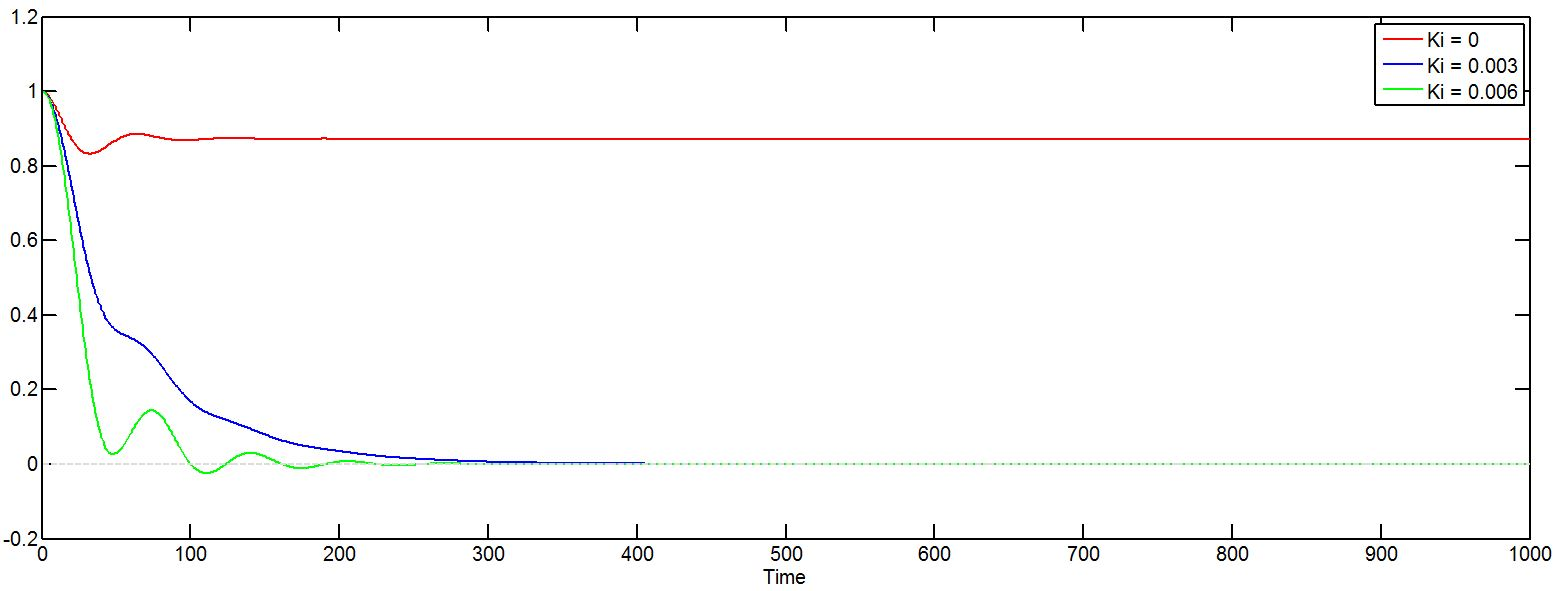
\includegraphics[scale=0.35]{images/PIDcontrol.jpg}
\caption{Example of proportional integral derivative controller}
\label{fig:PID_controller_example}
\end{figure}

To illustrate the steady-state error one of the values of $K_i$ is chosen to be zero. The highest value of the gain results in a small overshoot but reduces the error fast. The value in the middle results in no overshoot but reduces the error a bit slower. \\

As the example illustrates the PID controller were able to eliminate the error for the self-driving car and get it back on the right path.

% subsection integral_control (end)

% section pid_control (end)